\begin{frame}{Energy and momentum of pool balls}


  \begin{mycolumns}

    \begin{column}{.4\textwidth}\includegraphics[width=4in]{ch06/figs/pool-balls-energy-momentum}\end{column}

    \begin{column}{.6\textwidth}

      The cue ball hits the 10 ball. The cue ball stops dead, and the 10 ball flies off.
      Discuss this collision in terms of conservation of energy and momentum.

    \end{column}
  \end{mycolumns}

\end{frame}

\begin{frame}{Energy and momentum in different frames}


  \begin{mycolumns}

    \begin{column}{.4\textwidth}\includegraphics[width=4in]{ch06/figs/pool-balls-energy-momentum}\end{column}

    \begin{column}{.6\textwidth}

      The figure duplicates the earlier one, which we implicitly assumed to have been drawn in the frame of
      the felt surface of the pool table. Now imagine switching to a frame that is initially moving to the
      right along with the cue ball, and that continues moving at that speed after the collision (since we want
      it to be an inertial frame of reference). How does the analysis play out?

    \end{column}
  \end{mycolumns}

\end{frame}

\begin{frame}{In the middle}


  \begin{mycolumns}

    \begin{column}{.4\textwidth}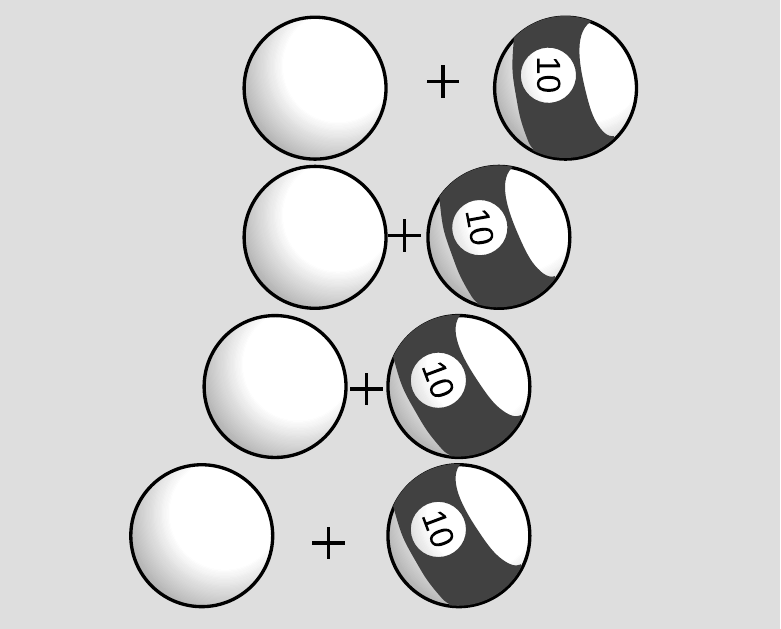
\includegraphics[width=4in]{ch06/figs/pool-balls-energy-momentum-cm}\end{column}

    \begin{column}{.6\textwidth}

      The collision is as before. The crosshairs trace the midpoint between the two balls. Consider the frame
      of reference you would get with a video camera that moved so as to keep the crosshairs centered.
      Work out the analysis in this frame.

    \end{column}
  \end{mycolumns}

\end{frame}

\begin{frame}{Pictures to words}


  \begin{mycolumns}

    \begin{column}{.3\textwidth}\includegraphics[width=3in]{ch06/figs/to-words-1}\end{column}

    \begin{column}{.7\textwidth}

      Interpret the process shown in the spacetime diagram.

    \end{column}
  \end{mycolumns}

\end{frame}

\begin{frame}{Pictures to words}


  \begin{mycolumns}

    \begin{column}{.3\textwidth}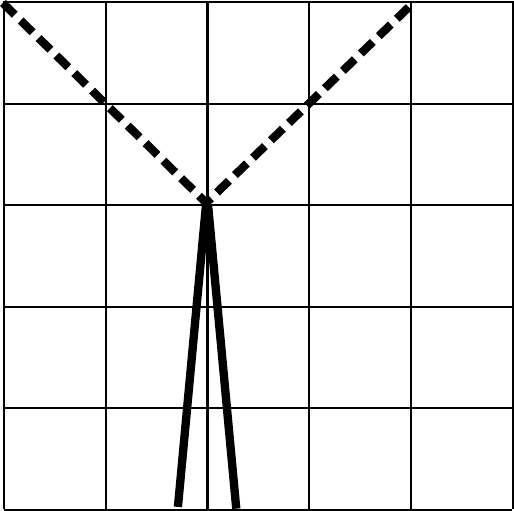
\includegraphics[width=3in]{ch06/figs/to-words-2}\end{column}

    \begin{column}{.7\textwidth}

      Interpret the process shown in the spacetime diagram.

    \end{column}
  \end{mycolumns}

\end{frame}

\begin{frame}{Pictures to words}


  \begin{mycolumns}

    \begin{column}{.3\textwidth}\includegraphics[width=3in]{ch06/figs/to-words-3}\end{column}

    \begin{column}{.7\textwidth}

      Interpret the process shown in the spacetime diagram.

    \end{column}
  \end{mycolumns}

\end{frame}

\begin{frame}{Impossible}


  \begin{mycolumns}

    \begin{column}{.3\textwidth}\includegraphics[width=3in]{ch06/figs/impossible-1}\end{column}

    \begin{column}{.7\textwidth}

      Use a law of physics to explain why the process is impossible.

    \end{column}
  \end{mycolumns}

\end{frame}

\begin{frame}{Impossible}


  \begin{mycolumns}

    \begin{column}{.3\textwidth}\includegraphics[width=3in]{ch06/figs/impossible-2}\end{column}

    \begin{column}{.7\textwidth}

      Use a law of physics to explain why the process is impossible.

    \end{column}
  \end{mycolumns}

\end{frame}

\begin{frame}{Impossible}


  \begin{mycolumns}

    \begin{column}{.3\textwidth}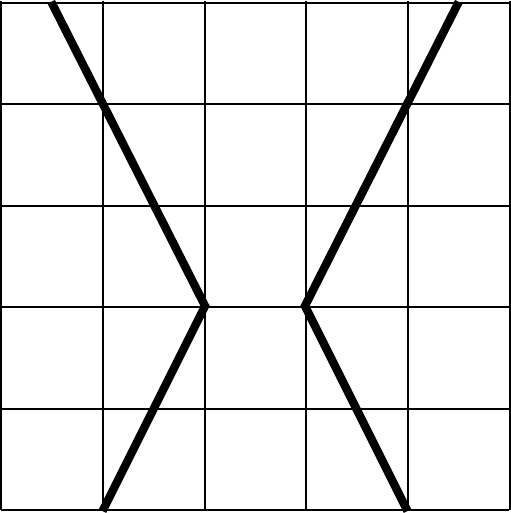
\includegraphics[width=3in]{ch06/figs/impossible-3}\end{column}

    \begin{column}{.7\textwidth}

      Use a law of physics to explain why the process is impossible.

      Hint: Consider it according to an observer who uses a different frame of reference, and has a different
      idea of simultaneity.

    \end{column}
  \end{mycolumns}

\end{frame}
